This chapter is constructed based on the published paper~\cite{yoneda2022}.

\section{Introduction}

The coupled phase-oscillator model is a mathematical model that describes the dynamics of a system of coupled oscillators. It is commonly used in the study of synchronization phenomena~\cite{strogatz2003}, such as the coordinated behavior of neurons in the brain~\cite{cossart2003,winfree1967,Lu2016} or the synchronized flashing of fireflies~\cite{smith1935,buck1968}. The model consists of a set of oscillators, each with its own phase, which are coupled through various forms of interactions, such as direct coupling or global coupling. The dynamics of the system are governed by a set of coupled differential equations, which can be analyzed to study the emergence of collective behavior and the effects of different coupling mechanisms on the oscillators' synchronization~\cite{kori2011}. This model has been widely applied in various fields, including physics~\cite{wang1988} and biology~\cite{Lu2016}, to gain insight into the mechanisms underlying synchronization in complex systems.

The estimation of equations describing rhythmic phenomena from data is a crucial step in understanding the underlying mechanisms of these phenomena. Revealing the equation of a rhythmic phenomenon can provide valuable insights into the behavior of the system and its properties. Many studies have been conducted to estimate the parameters of oscillator systems from data using methods such as Fourier series expansion. This approach has been widely applied in the study of rhythmic phenomena and has yielded important results in fields such as neuroscience and engineering.

The Bayesian linear regression formulation has been successfully applied to estimate the coefficients of the Fourier series, which is commonly used to represent the coupling function in oscillator systems~\cite{ota2014}. However, the order of the Fourier series, which determines the accuracy of the approximation, is typically arbitrary and subject to the limitations of the evidence approximation. Furthermore, the finite order approximation of the Fourier series may introduce oscillatory errors known as the Gibbs phenomenon, which can affect the accuracy of the estimates. 

One potential solution to the limitations of the Bayesian linear regression approach is to use Gaussian process regression, which offers greater flexibility in estimating the coupling function of the phase oscillator. Gaussian process regression is a non-parametric regression method that allows for the flexible modeling of complex functions through the use of a kernel function~\cite{rasumussen2006}. This kernel function can be designed to capture the smoothness, periodicity, and additive nature of the coupling function, enabling us to estimate the underlying dynamics of the phase oscillator system accurately~\cite{kanagawa2018}. In this chapter, we will introduce the concept of Gaussian process regression and demonstrate its effectiveness in estimating the coupling function of the phase oscillator.


This chapter is organized as follows.
% In Sec.~\ref{sec:preliminaries}, we briefly review coupled phase-oscillator models and Gaussian process regression.
In Sec.~\ref{sec:method}, we propose a method for extracting the coupling functions of oscillator systems from data exhibiting rhythmic phenomena using Gaussian process regression. This allows for more flexible estimation than Bayesian linear regression.
The proposed method is applied to equation 1 and equation 2 in the next Section~\ref{sec:numerical}.
Finally, we conclude this chapter and give some remarks in Sec.~\ref{sec:paper06_conclusion}.


\section{Problem setting}

In this chapter, we consider the general coupled limit-cycle oscillator models and predict the coupling functions of their reduced coupled phase-oscillator models from the phase data.
General coupled phase-oscillator models consist of $N$ oscillators with their phase $\theta_{i}$, and is governed by the following ODE,
\begin{align}
    \frac{\diff \theta_{i}}{\diff t}=\Gamma_{i}(\theta_{1}-\theta_{i},\ldots,\theta_{N}-\theta_{i}),
\end{align}
for $i=1,\ldots,N$.
The domain of a $i^{\mathrm{th}}$ coupling function $\Gamma_{i}$ is $N-1$ dimensional torus $\mathbb{T}^{N-1}$,
and each entry is the phase difference with another oscillator.
Therefore, our problem is to predict the coupling function $\Gamma_{i}\colon\mathbb{T}^{N-1}\to\mathbb{R}$ from data $\mathcal{D}=\{(\bm{x}_{j},y_{j})\}_{j=1}^{n_{\mathrm{data}}}$ with $\bm{x}_{j}\in\mathbb{T}^{N-1}$ and $y_{j}\in\mathbb{R}$ for $j=1,2,\ldots,n_{\mathrm{data}}$.

\section{Methodology: Gaussian process}
\label{sec:method}
In this chapter, we use the Gaussian process for regression and predict the coupling function.
We briefly address the procedure of the Gaussian process regression followed by the definition of Gaussian process.

% In conclusion, Gaussian process regression is a powerful and flexible method for estimating complex functions from data. Its ability to provide uncertainty estimates and incorporate prior knowledge make it a valuable tool in a wide range of applications, including the estimation of coupling functions in coupled phase oscillator systems.

\subsection{Gaussian process}
Gaussian process is a type of stochastic processes, and it is defined as follows:
\begin{define}[Gaussian process]
A stochastic process $\{X_{t}\}_{t\in T}$ is said to be a \textbf{Gaussian process}
if for any finite slices of index set $T$, say $(t_{1},\dots,t_{k})$,
\begin{align}
    (X_{t_{1}}, X_{t_{2}}, \dots, X_{t_{k}})
\end{align}
becomes a $k$-dimensional Gaussian random variable.
\end{define}
In many cases the index set $T$ is infinite one, hence a sample of Gaussian process can be seen as a function.
When $f\colon\mathcal{X}\to\mathbb{R}$ is a Gaussian process, we define functions $m\colon\mathcal{X}\to\mathbb{R}, k\colon\mathcal{X}\times\mathcal{X}\to\mathbb{R}$ by calculating
\begin{align}
    &m(x)=\mathbb{E}[f(x)],\\
    &k(x,\tilde{x})=\mathbb{E}[(f(x)-m(x))(f(\tilde{x})-m(\tilde{x}))],
\end{align}
for any $x,\tilde{x}\in\mathcal{X}$.
We refer to the function $m$ as a \textbf{mean function} and to the function $k$ as a \textbf{covariance function}.
It is known that Gaussian process is completely characterized by the functions $m$ and $k$.
In the following, we define the Gaussian process by determining $m$ and $k$,
and we write a Gaussian process variable (function) $f$ as
\begin{align}
    f\sim\mathcal{GP}(m,k).
\end{align}

Let's say a function $f$ be a Gaussian process with $f\sim\mathcal{GP}(m,k)$.
For finite points $X=(x_{1},\dots,x_{n})^{\top}$,
\begin{align}
    \bm{f}=f(X)\coloneqq(f(x_{1}),\dots,f(x_{n}))^{\top}
\end{align}
obeys a $n$-dimensional Gaussian distribution with a mean $m_{X}$ and a covariance matrix $k_{XX}$, which read
\begin{align}
    &m_{X}=m(X)\coloneqq(m(x_1),m(x_2),\dots,m(x_n))^{\top},\\
    &k_{XX}=k(X,X)\coloneqq\begin{pmatrix}
        k(x_{1},x_{1}) & k(x_{1},x_{2}) & \cdots & k(x_{1},x_{n})\\
        k(x_{2},x_{1}) & k(x_{2},x_{2}) & \cdots & k(x_{2},x_{n})\\
        \vdots & \vdots & \ddots & \vdots \\
        k(x_{n},x_{1}) & k(x_{n},x_{2}) & \cdots & k(x_{n},x_{n})
    \end{pmatrix}.
\end{align}
This is a direct consequence of the definition and its characterization of Gaussian process.
Sampling functions of Gaussian process is done by sampling Gaussian distribution random variables with $\mathcal{N}(m_{X},k_{XX})$, and the procedure is summarized in Algorithm~\ref{alg:gp_sample}.
We also plot samples of Gaussian process in Fig.~\ref{fig:rbf-sample} using this algorithm.

\begin{figure}[htbp]
    \begin{algorithm}[H]
      \caption{A function sampling Gaussian process \texttt{GP\_SAMPLE}}
      \label{alg:gp_sample}
      \begin{algorithmic}
      \Input sampling points $X=(x_{1},\dots,x_{n})$
      \Input Gaussian process $\mathcal{GP}(m,k)$ \Comment{mean function $m(\cdot)$, covariance function $k(\cdot,\cdot)$}
      \Output values of a sample of function from $\mathcal{GP}(m,k)$ of $X$
      \Function{\texttt{GP\_SAMPLE}}{$X,\mathcal{GP}(m,k)$}
      \State calculate mean array $m_{X} \gets m(X)=(m(x_{1},\dots,m(x_{n})))^{\top}$
      \State calculate covariance matrix $k_{XX} \gets [k_{XX}]_{i,j}=(k(x_{i},x_{j}))_{i,j}$
      \State calculate Cholesky decomposition matrix $L\gets\texttt{cholesky}(k_{XX})$ % \Comment{$k_{XX}=LL^{\top}$}
      \State generate $N$ samples from the standard normal distribution $\bm{z}\gets\texttt{randn}(n)$
      % \State \Comment{$z_{i}\sim\mathcal{N}(0,1)$}
      \State calculate affine transformation $\bm{f}\gets m_{X}+L\bm{z}$ \Comment{$\bm{f}\sim\mathcal{N}(m_{X},k_{XX})$}
      \State \Return $\bm{f}$
      \EndFunction
      \end{algorithmic}
    \end{algorithm}
\end{figure}

\begin{figure}[htbp]
    \centering
    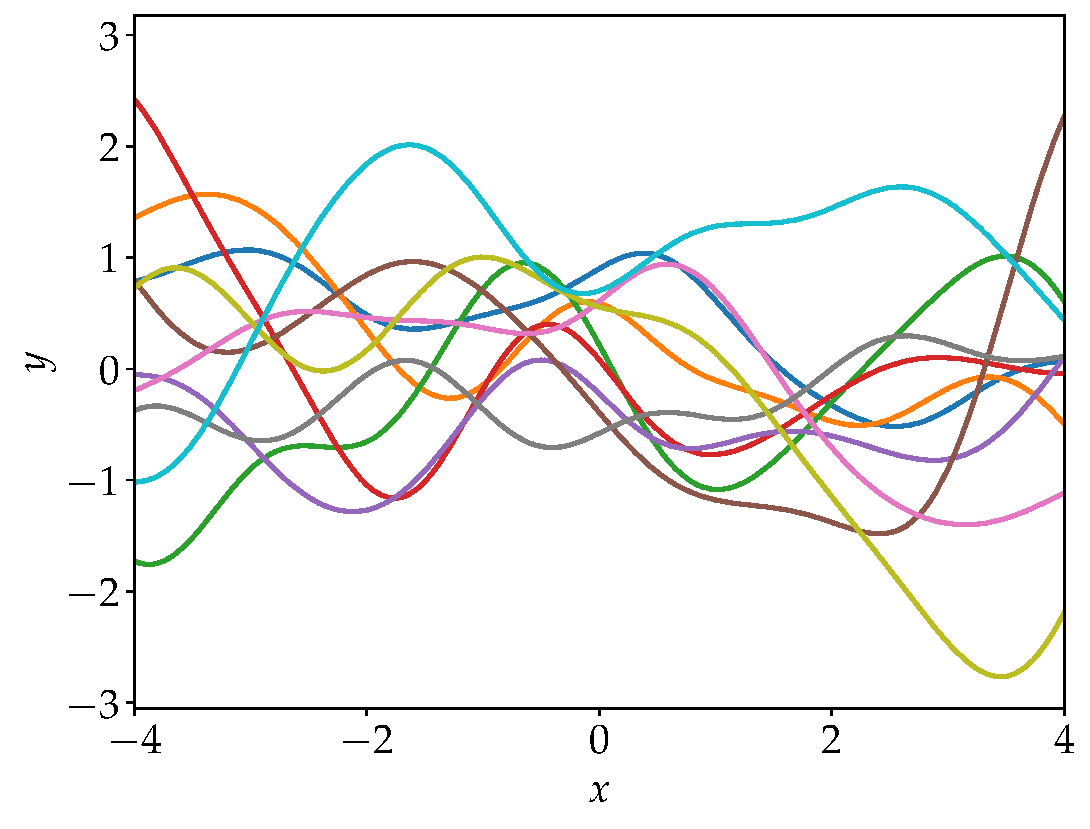
\includegraphics[width=0.7\textwidth]{figs/rbf_samples.pdf}
    \caption{Gaussian process sample paths.
    The mean function is $m(x)=0$ and the covariance function is $k(x,\tilde{x})=\exp[-(x-\tilde{x})^{2}/2]$.
    }
    \label{fig:rbf-sample}
\end{figure}


\subsection{Gaussian process regression}
Gaussian process regression is a non-parametric regression method that allows for the flexible modeling of complex functions. It is a Bayesian approach that uses a prior distribution over functions, which is updated based on the observed data to obtain a posterior distribution. The smoothness, periodicity, and additive nature of the function can be controlled through the use of a kernel function, which defines the covariance between different points in the function space.

One of the main merits of Gaussian process regression is its ability to provide uncertainty estimates for the regression parameters, which can be useful in situations where the data are noisy or sparse. It also allows for the modeling of complex functions without requiring the specification of a fixed functional form, which can be difficult to determine in many cases. Additionally, the use of a kernel function allows for the incorporation of prior knowledge about the function, such as its smoothness or periodicity, which can improve the accuracy of the estimates.

Let's say we have a data $\mathcal{D}=\{(\bm{x}_{j},y_{j})\}_{j=1}^{n_{\mathrm{data}}}\subset\mathcal{X}\times\mathbb{R}$ with $n_{\mathrm{data}}$ number of data and a function $f\colon\mathcal{X}\to\mathbb{R}$, such that
\begin{align}
    y_{i}=f(\bm{x}_{i})+\xi_{i},
\end{align}
for $i=1,\dots,n_{\mathrm{data}}$, where $\xi_{i}$ is a random variable of $\mathcal{N}(0,\sigma^{2})$ that represents a ``noise'' in the output.
Our task is to predict the unknown function $f$ from the data $\mathcal{D}$ using the Gaussian process.

We start by assuming that the unknown regression function $f$ is drawn from a given Gaussian process prior,
\begin{align}
    f\sim\mathcal{GP}(m, k),
\end{align}
where $m\colon\mathcal{X}\to\mathbb{R}$ is the mean function and $k\colon\mathcal{X}\times\mathcal{X}\to\mathbb{R}$ is the covariance function.
The covariance function $k$ should be chosen so that they reflect one’s prior knowledge or belief about the regression function $f$, and we will discuss this in the next subsection.
In many cases, the mean function $m$ is set to a constant zero function for simplicity.

The posterior distribution of $f$ is calculated analytically by linear algebra, and is again a Gaussian process. The distribution is given by the following closed form:
\begin{align}
    f\mid\mathcal{D}\sim\mathcal{GP}(\overline{m},\overline{k}),
\end{align}
where the posterior mean function $\overline{m}$ and the posterior covariance function $\overline{k}$ are
\begin{align}
    &\overline{m}(\bm{x})=m(\bm{x})+k_{\bm{x}X}(k_{XX}+\sigma^{2}I_{n_{\mathrm{data}}})^{-1}(\bm{y}-m_{X}),\\
    &\overline{k}(\bm{x},\bm{x}')=k(\bm{x},\bm{x}')-k_{\bm{x}X}(k_{XX}+\sigma^{2}I_{n_{\mathrm{data}}})^{-1}k_{X\bm{x}'}.
\end{align}
where $k_{XX}\in\mathbb{R}^{n_{\mathrm{data}}\times n_{\mathrm{data}}}$ denotes the matrix with elements $[k_{XX}]_{ij}=k(\bm{x}_{i},\bm{x}_{j})$,
$k_{X\bm{x}}=k_{\bm{x}X}^{\top}=(k(\bm{x}_{1},\bm{x}),\dots,k(\bm{x}_{n_{\mathrm{data}}},\bm{x}))^{\top}$,
$m_{X}=(m(\bm{x}_{1}),\dots,m(\bm{x}_{n_{\mathrm{data}}}))^{\top}$,
and $\bm{y}=(y_{1},\dots,y_{n_{\mathrm{data}}})^{\top}$.
We demonstrate the Gaussian process regression in Fig.~\ref{fig:gpr-sample}.
We see that the posterior mean function $\overline{m}$ is a good approximation of the true function.
\begin{figure}[htbp]
    \centering
    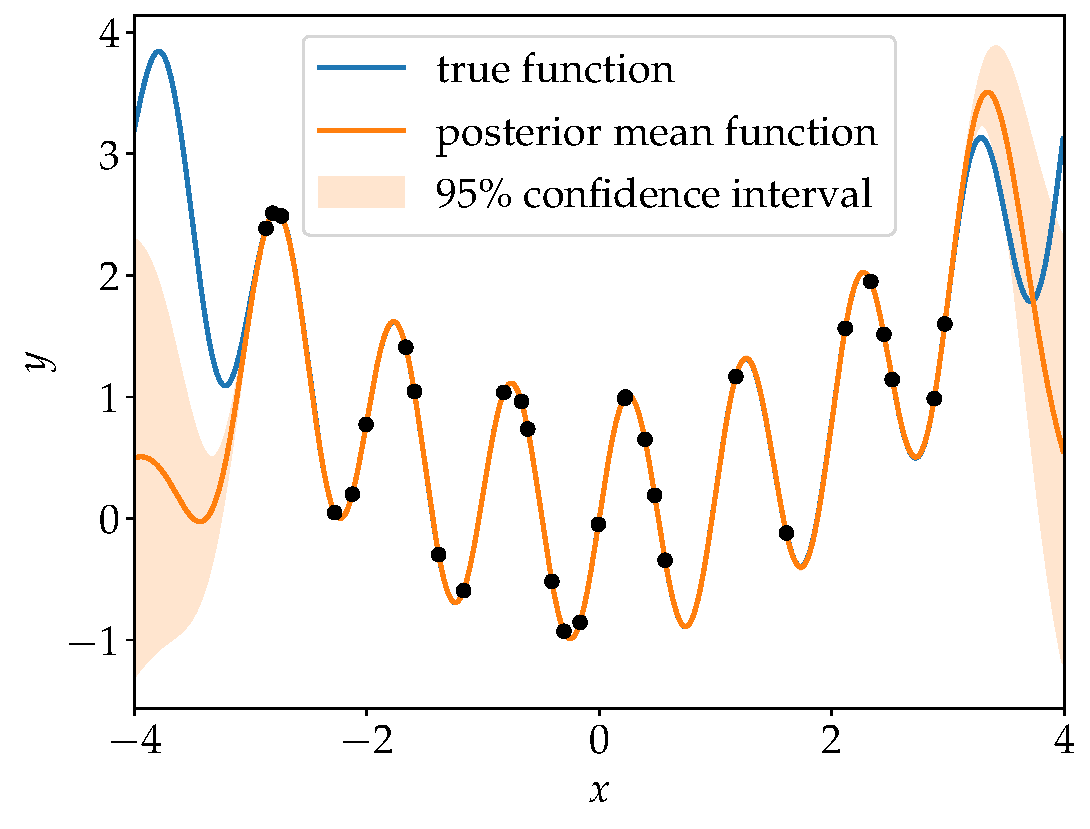
\includegraphics[width=0.7\textwidth]{figs/gpr_sample.pdf}
    \caption{Demonstration of Gaussian process regression.
    Black points denotes the data $\mathcal{D}=\{(x_{i},y_{i})\}_{i=1}^{30}$.
    The true function is $x\mapsto\sin(2\pi x)+x^{2}/5$.
    The prior mean function is $m(x)=0$ and the prior covariance function is $k(x,\tilde{x})=\exp[-(x-\tilde{x})^{2}/(2\sigma^{2})]$ with $\sigma=0.5$.}
    \label{fig:gpr-sample}
\end{figure}

Gaussian process regression has the advantage that all calculations can be done in a closed form using only matrix operations.
However, as the number of data $n_{\mathrm{data}}$ increases, inverse matrix calculations for $n_{\mathrm{data}}\times n_{\mathrm{data}}$ matrices are required, and the amount of memory and computation is enormous.
Many sparse approximations have been proposed to overcome the computational complexity of Gaussian process regression.
We give two examples of sparse approximations.
One is the sparse Gaussian process regression \cite{hensman2013}, which uses a subset of data as inducing variables.
Other is the sparse variational Gaussian process (SVGP) regression \cite{titsias2009}, which uses a variational distribution to approximate the posterior distribution of $f$.
Computation cost comparison is summarized in Table~\ref{table:gp-cost}.
In the following, we use the SVGP regression as our model.

\begin{table}[H]
    \caption{Computation cost comparison of Gaussian process regression.
    $n$ denotes the total number of data, $m$ denotes the number of inducing variables, and $b$ denotes the minibatch size.
    Sparse GP denotes the sparse Gaussian process regression \cite{hensman2013}, and SVGP denotes the sparse variational Gaussian process regression \cite{titsias2009}.}
    \label{table:gp-cost}
    \centering
    \begin{tabular}{l|cc>{\columncolor[rgb]{1.0,1.0,0.7}}c}
      & GP & sparse GP & SVGP \\\hline\hline
     Inference cost & $\mathcal{O}(n^{3})$ & $\mathcal{O}(nm^{2})$ & $\mathcal{O}(bm^{2}+m^{3})$ \\
     Memory cost & $\mathcal{O}(n^{2})$ & $\mathcal{O}(nm)$ & $\mathcal{O}(bm+m^{2})$ \\
    \end{tabular}
\end{table}



\subsection{Choice of a covariance function}

A covariance function is a crucial ingredient in a Gaussian process predictor, as it encodes our assumptions about the function which we wish to learn.
For example, the radius basis function (RBF) is known to generate a $C^{\infty}$ function with probability one.
Matérn covariance function is known to generate a finite-time differentiable function with probability one.
See \cite{kanagawa2018} for a detailed discussion.
In this chapter, the coupling function which we wish to learn has a domain of torus $\mathcal{X}=\mathbb{T}^{N-1}$.
When $N=2$, the domain is $\mathcal{X}=\mathbb{T}^{1}=\mathbb{S}^{1}$ and the coupling function is a simple periodic function.
By assuming that the function is smooth, we can set the covariance function as 
\begin{align}
    k(x,x')=\theta_{0}\exp(\theta_{1}\cos(x-x')),
    \label{eq:kernel-1d}
\end{align}
which is often called a \textit{periodic kernel}.
Here, $\theta_{0}$ and $\theta_{1}$ are positive hyperparameters.
$\theta_{0}$ determines the \textit{amplitude} of the covariance function,
and $\theta_{1}$ can be said as an \textit{inverse lengthscale},
which specifies the width of the covariance function.
Therefore $\theta_{1}$ determines the smoothness of the coupling function,
and it is important to choose an appropriate value of $\theta_{1}$.
In many cases, the hyperparameters are to set by maximizing the marginal likelihood,
and we will see this in the next subsection.
We demonstrate the heatmaping of the covariance function and the corresponding samples of Gaussian process in Fig.~\ref{fig:kernel-comparison}.

\begin{figure}[htbp]
    \centering
    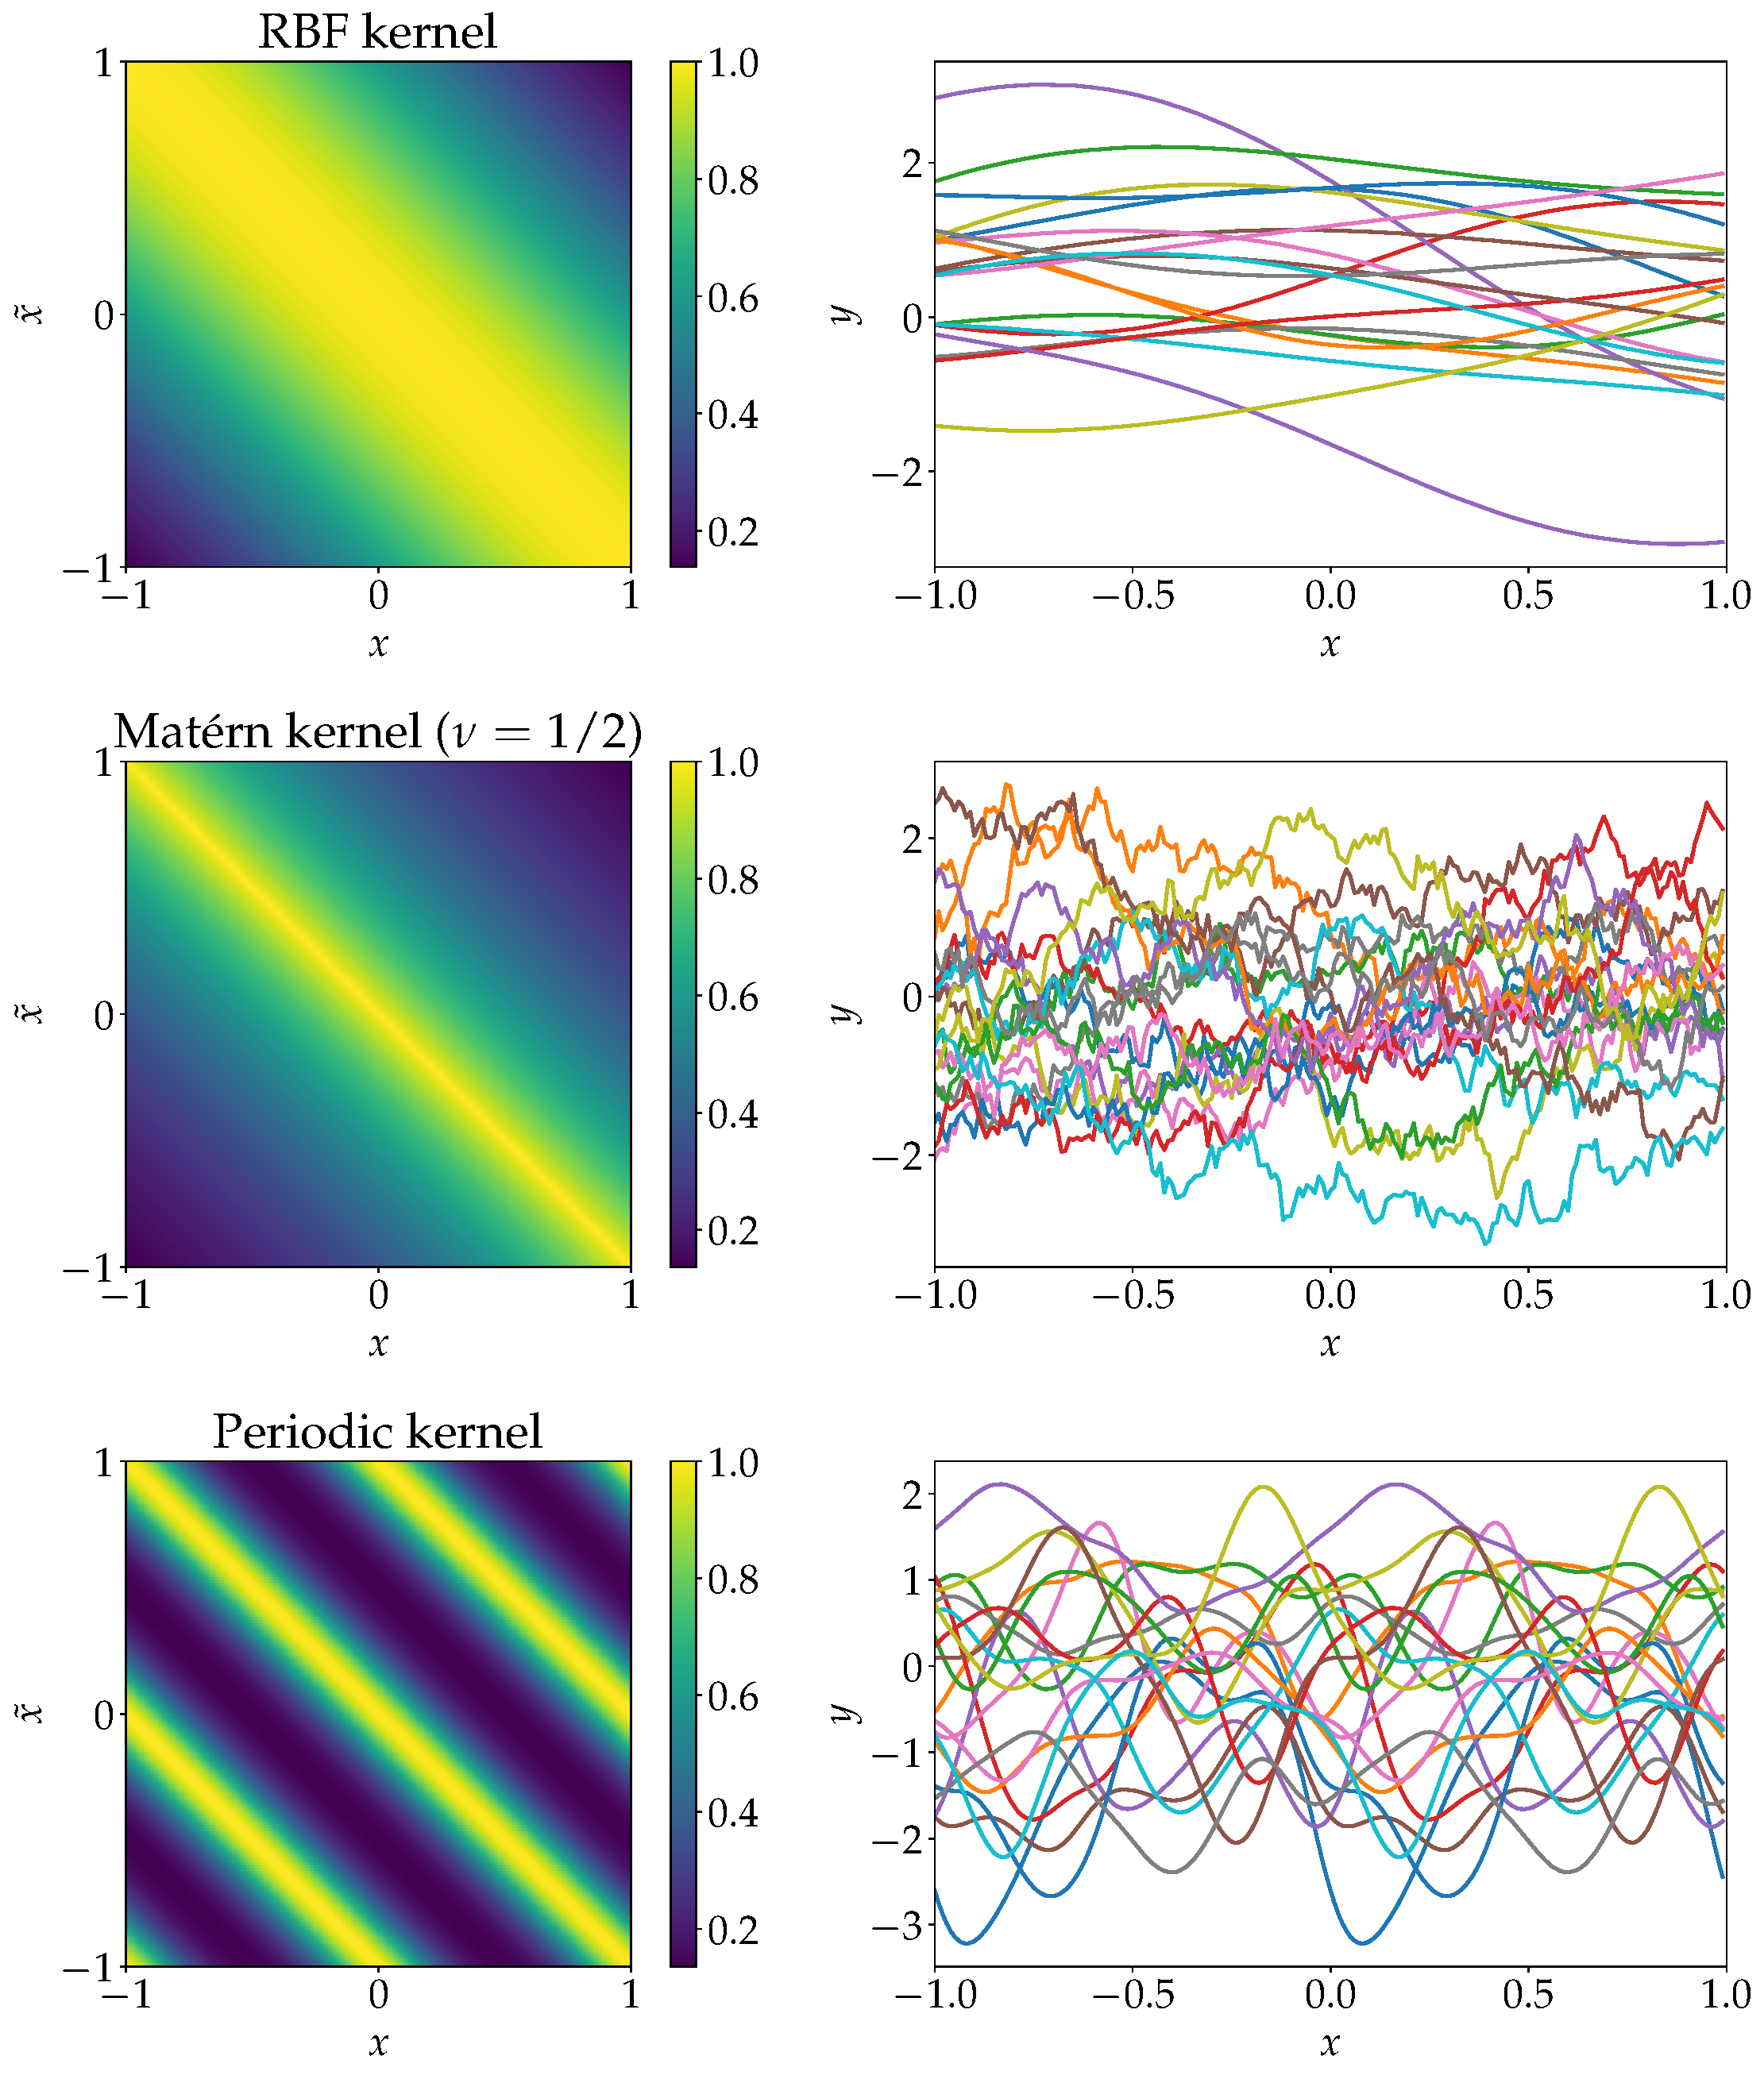
\includegraphics[width=\textwidth]{figs/kernel_comparison.pdf}
    \caption{
    (left) Heatmaps of the RBF kernel, Matérn kernel ($\nu=1/2$), and periodic kernel. (right) Samples of Gaussian process with the RBF kernel, Matérn kernel ($\nu=1/2$), and periodic kernel.
    }
    \label{fig:kernel-comparison}
\end{figure}

When $N\geq3$, the domain is defined on the product space $\mathcal{X}=\mathbb{S}^{1}\times\cdots\times\mathbb{S}^{1}$,
and the coupling function is expected to be periodic and smooth with respect to each entry of the domain.
We can construct the covariance function from \eqref{eq:kernel-1d} by tensor product as follows:
\begin{align}
    k(\bm{x},\bm{x}')=\theta_{0}\exp\left(\sum_{i=1}^{N-1}\theta_{1}^{(j)}\cos(x_{j}-x_{j}')\right),
\end{align}
where $\theta_{0},\theta_{1}^{(j)}$ are positive hyperparameters.

Some systems can further be reduced to coupled phase-oscillator models in the following ODE form called an \textit{additive model}:
\begin{align}
    \Gamma_{i}(\theta_{1}-\theta_{i},\ldots,\theta_{N}-\theta_{i})=\omega_{i}+\sum_{j\ne i}\Gamma_{ij}(\theta_{j}-\theta_{i}),
    \label{eq:cpo-additive}
\end{align}
which is a linear combination of functions of one variable~\cite{duvenaud2011,rasumussen2006}.
In this case, we can construct a covariance function which generates the additive model shown in \eqref{eq:cpo-additive}.
By assuming that each coupling function $\Gamma_{ij}$ is the periodic function of the phase difference and is smooth,
the covariance function of $\Gamma_{i}$ will have the form of a direct sum of periodic kernels, which reads
\begin{align}
    k(\bm{x},\bm{x}')=\sum_{j=1}^{N-1}\theta_{0}^{(j)}\exp\left(\theta_{1}^{(j)}\cos(x_{j}-x_{j}')\right),
\end{align}
where $\theta_{0}^{(j)},\theta_{1}^{(j)}$ are positive hyperparameters.

% \begin{figure}
%     \centering
%     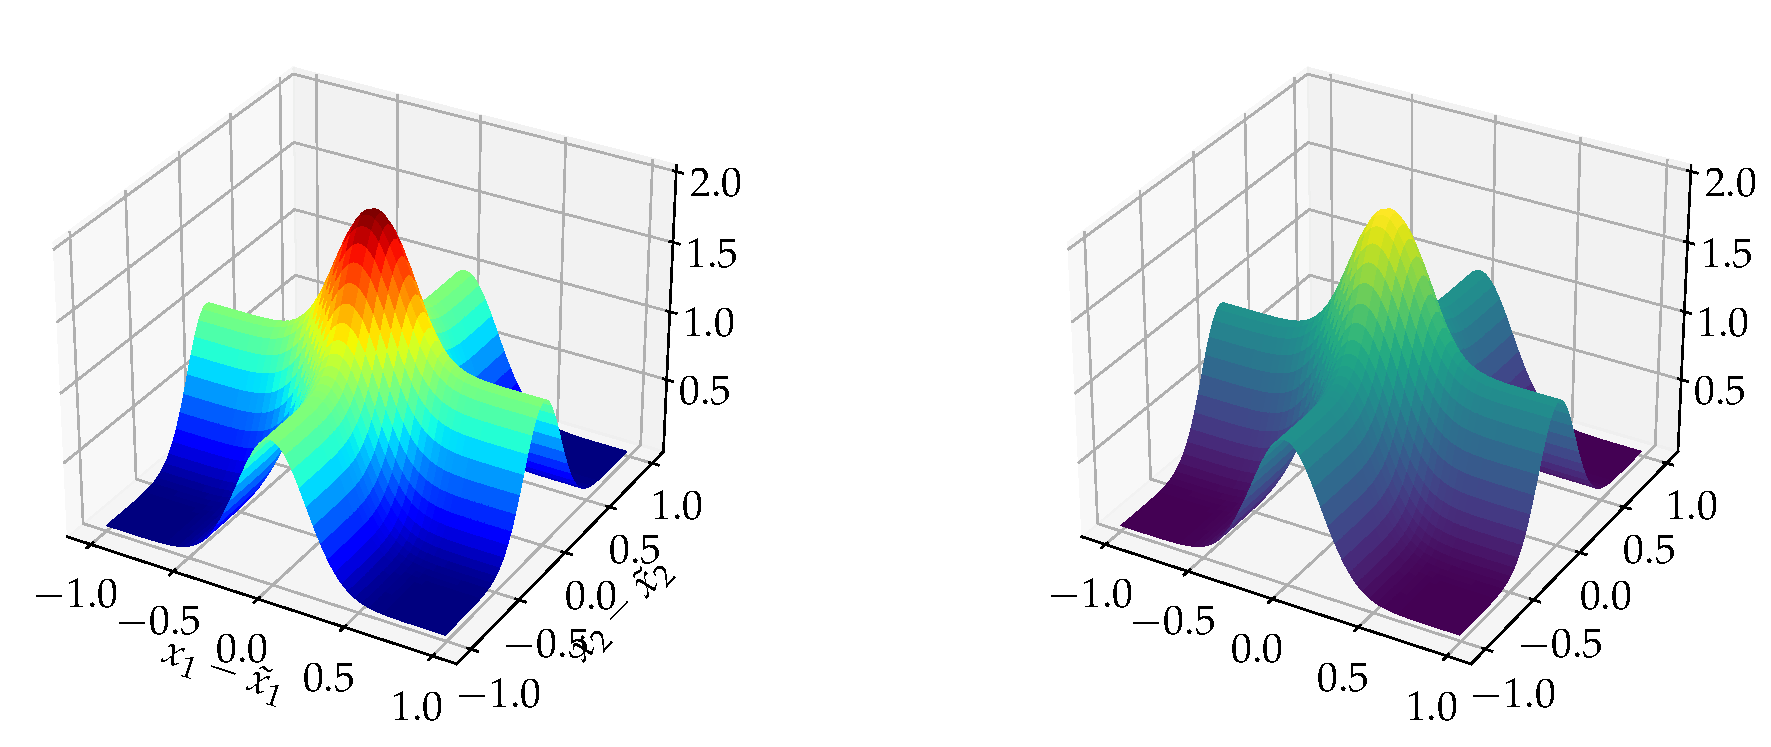
\includegraphics[width=\textwidth]{figs/additive_kernel.pdf}
%     \caption{hoge}
%     \label{fig:additive-kernel}
% \end{figure}

\subsection{Optimization}
In the Gaussian process regression described so far,
hyperparameters remain in the kernel $\theta_{0,1}$ and the noise strength $\sigma$.
For brevity of notation, we will write these parameters as $\bm{\theta}$.

To estimate $\bm{\theta}$, we consider the \textit{maximum likelihood estimation},
which makes inferences about the population that is most likely to have generated the data $\mathcal{D}$.
The (marginal) log-likelihood for parameters $\bm{\theta}$ is
\begin{align}
    \mathcal{L}(\bm{\theta})=\log p(\bm{y}\mid X, \bm{\theta})=-\frac{1}{2}\bm{y}^{\top}K_{\bm{\theta}}\bm{y}-\frac{1}{2}\log\det K_{\bm{\theta}}-\frac{n_{\mathrm{data}}}{2}\log 2\pi,
\end{align}
where $K_{\bm{\theta}}=k_{XX}+\sigma^{2}I_{n_{\mathrm{data}}}$ is the covariance matrix for the noisy data $\mathcal{D}$.
The most probable parameters $\bm{\theta}$ are, therefore, estimated by finding the maximum of the log-likelihood function $\mathcal{L}(\bm{\theta})$.

The problem of finding the point that maximizes the marginal likelihood while changing hyperparameters is formulated as an optimization problem.
In this chapter, we use the gradient descent method is to find the maximum point of the marginal likelihood.
The hyperparameters $\bm{\theta}$ is updated using the gradient with the following manner:
\begin{align}
    \bm{\theta}^{(t+1)} \leftarrow \bm{\theta}^{(t)} + \alpha\frac{\partial\mathcal{L}}{\partial\bm{\theta}}(\bm{\theta}^{(t)}),
\end{align}
where $\alpha$ denotes the learning rate.

Stochastic gradient decent (SGD) method, regarded as a stochastic approximation of gradient descent optimization methods, is another way of optimization.
In the SGD method, the gradient is determined by different minibatches at each step, and parameter updating proceeds accordingly.
The greatest benefit is that it requires less computation time to converge than the gradient method, which uses all data at each step.
It is also thought to be less likely to be trapped in local solutions, thanks to stochastic fluctuations in the gradient direction for each minibatch.

\section{Numerical Simulations}
\label{sec:numerical}

% \subsection{Coupled phase oscillators}
% We first consider the coupled phase-oscillator model,
% \begin{align}
% &\dot{\theta}_{1}=\dots,\\
% &\dot{\theta}_{2}=\dots,\\
% &\dot{\theta}_{3}=\dots,
% \end{align}

% \blue{3たいの結合振動子系を考える。この結合関数をデータから推定する。はじめにデータを生成する。初期点をランダムに決めて$t_{0}=0.0,t_{1}=15.0$の間をEuler法で解いて、っていうのを10回行う。このときデータ点は$N$個になる。得られたデータをもとに結合関数を推定する。このとき$\theta_{1}$のベクトル場を推定するにはガウス過程回帰を行うためのカーネル関数は
% \begin{align}
% k(\bm{x},\bm{y})=\theta_{0}^{(1\to 2)}\exp(\theta_{1}^{(1\to2)}\cos(x_{1}-y_{1}))+\theta_{0}^{(1\to 3)}\exp(\theta_{1}^{(1\to3)}\cos(x_{2}-y_{2}))
% \end{align}
% になる。カーネルに含まれるハイパーパラメータは4つである。}




\subsection{Coupled Van der Pol oscillators}
\label{subsec:vdp}
Next, we consider the Van der Pol equation, which is a mathematical model that describes the nonlinear dynamics of a damped oscillator~\cite{pol1926}. It is commonly used in the study of oscillator systems, such as those found in electrical circuits and mechanical systems. The equation takes the form:
\begin{align}
    &\dot{x}=y,\\
    &\dot{y}=\varepsilon(1-x^{2})y-x,
\end{align}
where $x$ and $y$ are the position and velocity of the oscillator, respectively,
and $\varepsilon$ is a constant that determine the damping and frequency of the oscillation. The equation exhibits a wide range of behavior, including limit cycles, bifurcations, and chaos, depending on the values of $\varepsilon$.

In this subsection, we connect two Van der Pol oscillators in the following manner:
\begin{align}
    &\dot{x}_{1}=y_{1}+K(x_{2}-x_{1})+\xi_{x_{1}}(t),\\
    &\dot{y}_{1}=\varepsilon_{1}(1-x_{1}^{2})y_{1}-x_{1}+Kx_{2}^{2}y_{2}+\xi_{y_{1}}(t),\\
    &\dot{x}_{2}=y_{2}-Kx_{1}^{2}y_{1}+\xi_{x_{2}}(t),\\
    &\dot{y}_{2}=\varepsilon_{2}(1-x_{2}^{2})y_{2}-x_{2}+Kx_{1}y_{1}^{2}+\xi_{y_{2}}(t),
\end{align}
where $\xi_{\alpha}(t)$ are Gaussian white noises with $\langle\xi_{\alpha}(s)\xi_{\beta}(t)\rangle=\sigma^{2}\delta_{\alpha,\beta}\delta(s-t)$ for $\alpha,\beta\in\{x_{1},y_{1},x_{2},y_{2}\}$.
Parameter values are $\varepsilon_{1}=0.3,\varepsilon_{2}=0.7,K=0.01,\sigma=0.03$.

We first obtain the oscillators' orbit by numerically integrating the equations using Euler--Maruyama method.
We use the position values $x_{1,2}$ as observables of the Van der Pol oscillators.
These values are different from the phase representation, and we need to transform to phases.
In this chapter, we use the Hilbert transformation, which transform the real valued function $u(t)$ to another real valued $\mathcal{H}[u](t)$, and calculate the argument of complex $u(t)+i\mathcal{H}[u](t)$ as the phase function of time $t$.
However, this method has the problem that the phase does not vary monotonically when there is no interaction or noise.
Therefore, we transform the phase using the method proposed by Kralemann as the following:
\begin{align}
    \phi[\theta](t)=2\pi\int_{0}^{\theta}f(\theta)\diff\theta,
\end{align}
where $f(\theta)$ denotes the probability distribution of time series $\theta$~\cite{kralemann2011,kralemann2008,kralemann2007}.
After these procedures, we obtain the time series of phases in the following form:
\begin{align}
\begin{bmatrix}
    \theta_{1}(t_{1}) & \theta_{1}(t_{2}) & \cdots & \theta_{1}(t_{k})\\
    \theta_{2}(t_{1}) & \theta_{2}(t_{2}) & \cdots & \theta_{2}(t_{k})
\end{bmatrix}.
\end{align}
Since our goal is to do the regression for coupling functions, we create input-output data from the phase time series $\mathcal{D}$ for each dimension.
For the firs oscillator, we set the data $\mathcal{D}=\{(x_{i},y_{i})\}_{i=1}^{n_{\mathrm{data}}}$ with
\begin{align}
    x_{i}=\theta_{2}(t_{i})-\theta_{1}(t_{i}),\quad y_{i}=\frac{\theta_{1}(t_{i+1})-\theta_{1}(t_{i})}{t_{i+1}-t_{i}},
\end{align}
where $y_{i}$ is approximation of time differentiation of $\theta_{1}$ at time $t_{i}$ using the finite time difference. For simplicity, $x_{i},y_{i}$ are used here as variables, which are different from the variables in the original Van der Pol equations.

Now we have the input-output data $\mathcal{D}$ for the coupling funtion, we conduct the Gaussian process regression.
We especially use the stochastic variational Gaussian process regression for lighter computation cost compared to the original Gaussian process regression approach.
Since total number of oscillators are two, the input dimension of the coupling function is one, and the covariance fucntion for the Gaussian process regression should take the form:
\begin{align}
    k(x,\tilde{x})=\theta_{0}\exp[\theta_{1}\cos(x-\tilde{x})],
\end{align}
for $x,\tilde{x}\in\mathbb{S}^{1}$.
Parameters $\theta_{0,1}>0$ are optimized by Adam optimizer in the stochastic variational Gaussian process regression learning process~\cite{titsias2009,kingma2014}.
The result is shown in Fig.~\ref{fig:vdp_gp}, comparing with the true coupling function and the 
The Gaussian process regression approach successfully obtains the coupling function.

\begin{figure}[htbp]
    \centering
    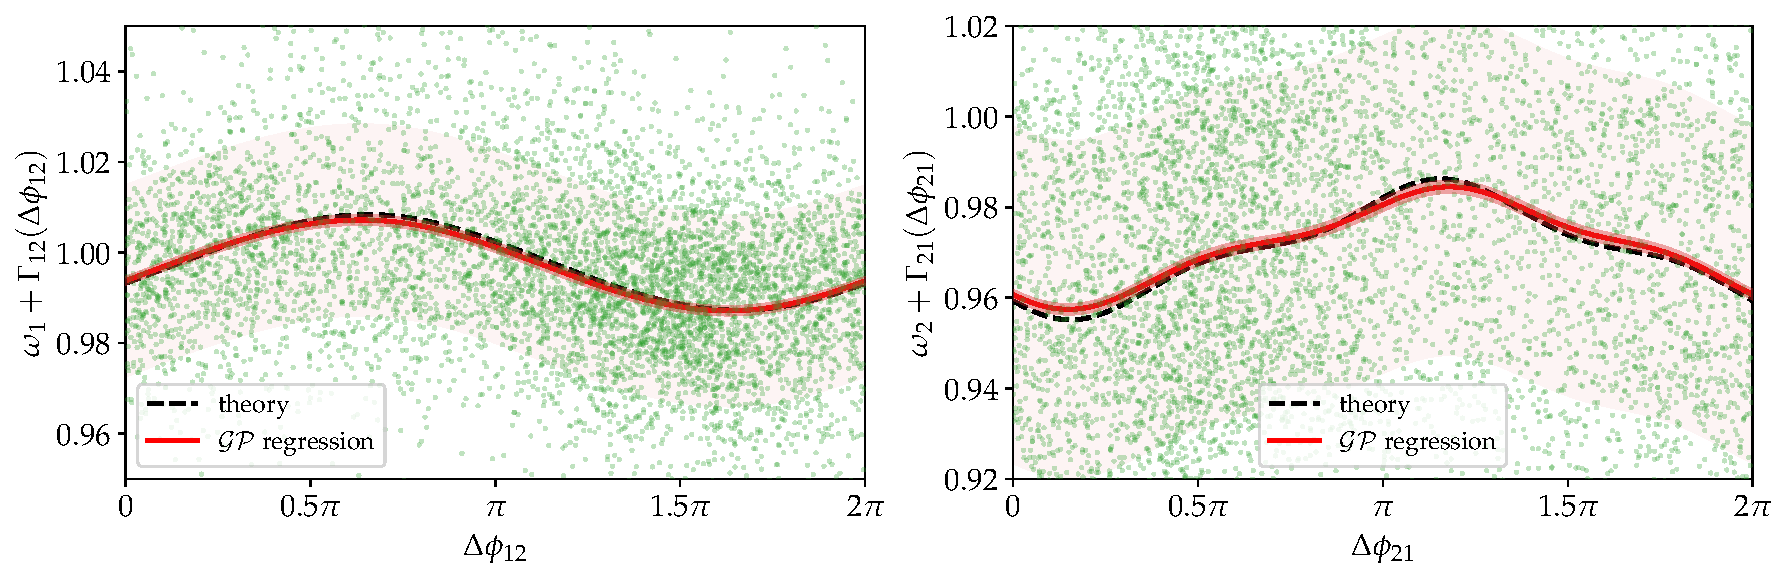
\includegraphics[width=\textwidth]{figs/vdp_gp.pdf}
    \caption{Estimation of the coupling functions of the Van der Pol oscillators.
    The Gaussian process approach is compared to the theory plot, which is obtained by the phase reduction theory.
    Green dots are the data points used for the Gaussian process regression.
    Dark red bars are the standard deviation of the Gaussian process regression with respect to the estimated function, and pale red bars are the standard deviation of the Gaussian process regression with respect to the data points.
    }
    \label{fig:vdp_gp}
\end{figure}

We also give a situation where the previous method, using the Fourier series expansions, fails to estimate the coupling function while the Gaussian process regression approach succeeds in Fig.~\ref{fig:gp_fourier_comparison}.
We estimate the coupling function of the Van der Pol oscillators for the second oscillator with the same parameters as the previous example.
The Fourier series expansion approach fails to choose the appropriate number of degrees through the evidence approximations.
On the other hand, the Gaussian process regression approach is non-parametric,
hence it can focus only on the estimation of the coupling function without worrying about the number of degrees.

\begin{figure}[htbp]
    \centering
    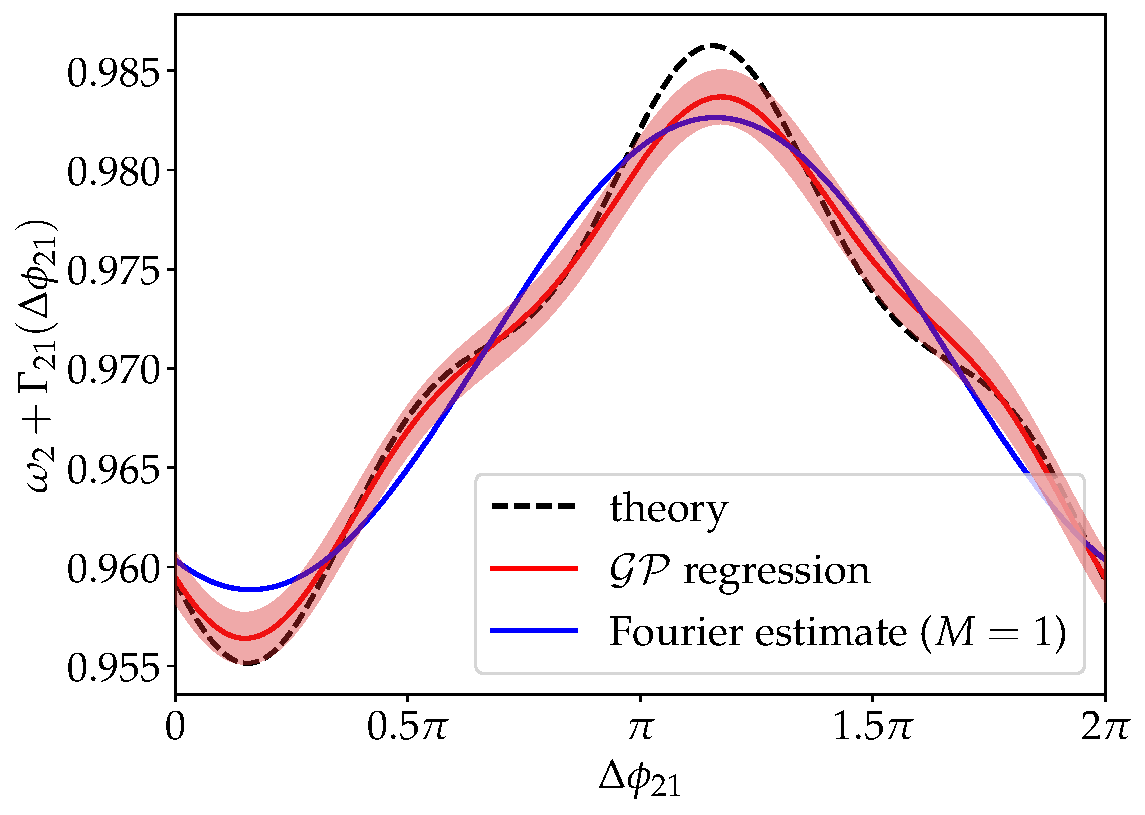
\includegraphics[width=0.8\textwidth]{figs/gp_fourier_comparison.pdf}
    \caption{
        Comparison of the Fourier series and the Gaussian process regression.
    }
    \label{fig:gp_fourier_comparison}
\end{figure}

\subsection{Spiking Neural Network oscillators}

We next estimate the network of seven neuron oscillators.
The network consists of five excitatory neurons, which is modeled by Hodgkin--Huxley model~\cite{hodgkin1952},
and two inhibitory neurons, which is modeled by fast spiking neuron model~\cite{erisir1999}.
Details of these models are summarized in Appendix~\ref{sec:neuron-model}.
See the upper left network plot in Fig.~\ref{fig:snn}.
We observe the time series by numerically solving the equations of spiking neurons (which is shown in Appendix~\ref{sec:neuron-model}), and use the membrane voltages $V_{i}(t)$ for the regression.
Time series of the membrane voltages are shown in the upper right of Fig.~\ref{fig:snn}.
We apply the same procedures as done in Sec.~\ref{subsec:vdp} and get the phase time series, which takes the following form:
\begin{align}
\begin{bmatrix}
    \theta_{1}(t_{1}) & \theta_{1}(t_{2}) & \cdots & \theta_{1}(t_{k})\\
    \theta_{2}(t_{1}) & \theta_{2}(t_{2}) & \cdots & \theta_{2}(t_{k})\\
    \vdots & \vdots &  & \vdots\\
    \theta_{7}(t_{1}) & \theta_{7}(t_{2}) & \cdots & \theta_{7}(t_{k})
\end{bmatrix}.
\end{align}
For the first oscillator, we set the data $\mathcal{D}=\{(\bm{x}_{i},y_{i})\}_{i=1}^{n_{\mathrm{data}}}$ with
\begin{align}
    \bm{x}_{i}=\begin{bmatrix}
        \theta_{2}(t_{i})-\theta_{1}(t_{i})\\
        \theta_{3}(t_{i})-\theta_{1}(t_{i})\\
        \vdots\\
        \theta_{7}(t_{i})-\theta_{1}(t_{i})
    \end{bmatrix}\in\mathbb{T}^{6},\quad
    y_{i}=\frac{\theta_{1}(t_{i+1})-\theta_{1}(t_{i})}{t_{i+1}-t_{i}}.
\end{align}
Since the input space in $\mathbb{T}^{6}$, the covariance function for the Gaussian process regression is
\begin{align}
    k(\bm{x},\tilde{\bm{x}})=\sum_{j=1}^{6}\theta_{0}^{(j)}\exp(\theta_{1}^{(j)}\cos(x_{i}-\tilde{x}_{i})),
\end{align}
for $\bm{x},\tilde{\bm{x}}\in\mathbb{T}^{6}$.
For this input-output data, we employ the stochastic variational Gaussian process regression and estimate the first oscillator's coupling function.
We simultaneously estimate the coupling functions for other oscillators.
See the lower graphs of Fig.~\ref{fig:snn} for the estimation result compared to the theoretical coupling functions obtained by the phase reduction approach.
We confirm that the coupling functions between each oscillators are qualitatively consistent with the results from Gaussian process regression and the theoretical results.

\begin{figure}[htbp]
    \centering
    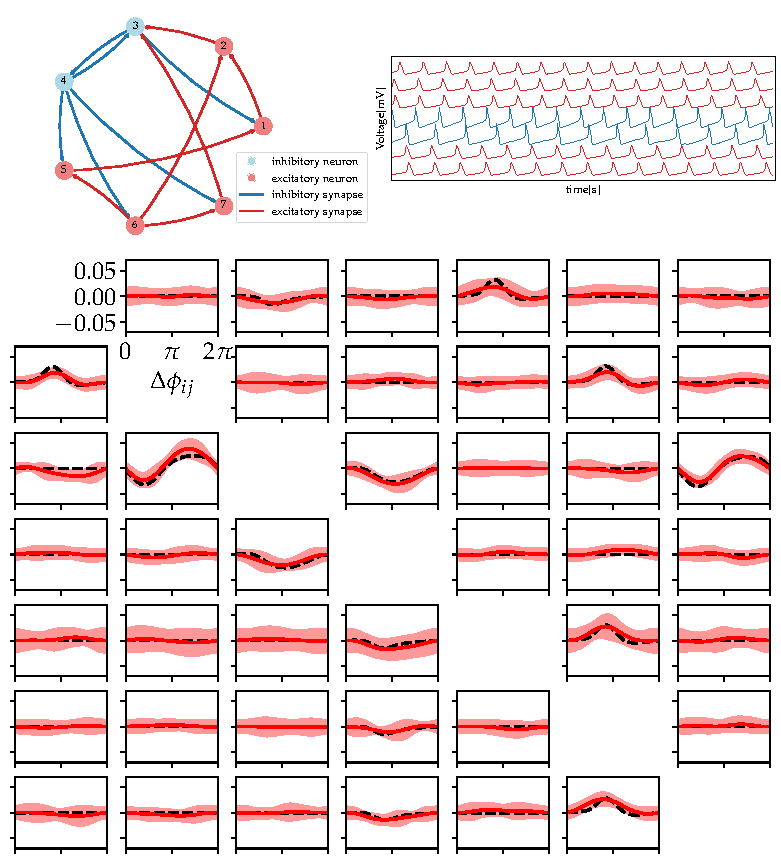
\includegraphics[width=\textwidth]{figs/snn.pdf}
    \caption{(Upper left) Network of spiking neurons coupled with inhibitory and excitatory neurons. (Upper right) Time series of the voltage of each neuron. (lower) Theoretically derived coupling function between each neuron (black dotted line) and the coupling function estimated from the data using Gaussian process regression (red solid line). Red bars are the standard deviation of the Gaussian process regression with respect to the estimated functions.
    Note that for comparison each coupling function $\Gamma_{ij}$ is translated to take $0$ at $\Delta\phi_{ij}=0$.}
    \label{fig:snn}
\end{figure}

\section{Summary and Discussions}
\label{sec:paper06_conclusion}
In this chapter, we focus on the real data that represent rhythmic phenomena, and from them, we consider estimating the coupling function that is modeled as a phase oscillator system. A method for estimating the coupling function using Gaussian process regression is proposed. By designing the kernel function flexibly, the regression can be performed without going through a finite order approximation by Fourier series. We confirmed that this works well in the case of Van der Pol equations. We also confirmed that the coupling function can be successfully estimated qualitatively for as many as seven many-body systems of coupled spiking neurons.

Finally, we comment on the proposed method using Gaussian process regression. The main idea was to reduce the data to a regression problem about a vector field of differential equations of phase. However, the possibility arises that the data used in the regression may contain systematic errors because it involves an approximation of the derivative in terms of differences due to finite time. To overcome this problem, a new idea has recently been proposed to calculate the parameter derivatives of time series data obtained from parameterized vector fields using the accompanying equations~\cite{chen2018,li2020}. We leave the application of the adjoint equation to the estimation of coupling functions as a future work.
